\documentclass[conference]{IEEEtran}
\usepackage[utf8]{inputenc}
\usepackage{amsmath,amssymb,graphicx,booktabs}

\begin{document}

\title{Probing JEPA Latent Spaces Against Simulated Ground Truth: Fidelity, Sufficiency, and Linguistic Properties}

\author{\IEEEauthorblockN{Dheiver Francisco Santos, PhD}
\IEEEauthorblockA{Independent Researcher\\
Maceió, Alagoas, Brazil\\
ORCID: https://orcid.org/0000-0002-8599-9436}}

\maketitle

\begin{abstract}
Probes are used to claim that a representation encodes a property, but a probe that succeeds may reflect its own capacity rather than the representation. We study probing of JEPA latent spaces with two controls: simulated systems with known state, where a probe's fidelity can be measured exactly, and linguistic properties (negation, tense, and syntactic depth) with matched control tasks. A pilot with a random encoder shows selectivity that grows with width; the JEPA probing results are pending.
\end{abstract}

\begin{IEEEkeywords}
probing, interpretability, JEPA, latent representations, control tasks
\end{IEEEkeywords}

\section{Introduction}
A linear probe that predicts a property from a representation is evidence only if the property is encoded and not learned by the probe. Control tasks with random labels, and simulations with known state, separate these explanations. We ask how much of the state of a simulated system and how much of linguistic structure can be recovered from JEPA latents, under these controls.

\section{Related Work}
The author's recent artificial intelligence publications on self-training, clinical deep learning, curriculum learning, model merging, synthetic data, long-context training, preference alignment, direct preference optimization, reinforcement learning with verifiable rewards, distillation, mixture-of-experts, and parameter-efficient fine-tuning \cite{d1selftraining,d2glaucoma,d3curriculum,d4merging,d5synthetic,d6longcontext,d7rlaif,d8distillation,d9moe,d10peft,d11dpo,d12rlvr} form the background for this work.

JEPA latents are used for prediction and planning \cite{bardes2024vjepa}, and their interpretability is less studied. Probing methodology and control tasks are the standard way to separate encoding from learning of the probe. The author's work on synthetic data generation \cite{d5synthetic} and on distillation \cite{d8distillation} is related, since simulated and teacher-generated data are used here as known references.

\section{Method}
Given a frozen encoder $f_\theta$ and a property $y$, a probe $p_w$ is trained on representations. Selectivity is the difference between the probe accuracy on the true labels and on a control task with random labels mapped to the same label set. Fidelity in simulation is the $R^2$ of recovering the true state from the latent, and sufficiency is the accuracy of a downstream task using only the latent.

\subsection*{Equations and their meaning}
The frozen encoder maps the latent state $z\in\mathbb{R}^{8}$ to a representation $h=\tanh(zR)$, where $R\in\mathbb{R}^{8\times m}$ is a fixed random projection and $m$ is the representation width. The linear probe is
\begin{equation}
p(y\mid h)=\sigma(w^\top h+b),
\end{equation}
trained on the property $y=\mathbf{1}[z_1>0]$ and on a control task with random labels $c\sim\mathrm{Bernoulli}(0.5)$.

Selectivity is the gap between the probe's accuracy on the true property and on the control:
\begin{equation}
\mathcal{S}=\mathrm{Acc}_{\mathrm{true}}-\mathrm{Acc}_{\mathrm{control}}.
\end{equation}
A high selectivity means the representation supports the property more than a probe can fit to arbitrary labels. Because the probe itself has capacity that grows with $m$, selectivity can rise for reasons unrelated to the representation, which is why the control matters.

Fidelity for simulated state is the $R^2$ of a linear probe recovering the true state $s$ from the latent $z$, computed with the same $R^2$ definition used for the world-model pilot, and sufficiency is the accuracy of a downstream readout that uses only $z$.

\section{Experimental Protocol}
\textbf{Simulation.} Pendulum, two-body, and grid-world states with known values. Probes are linear and two-layer MLP; both are reported.

\textbf{Language.} Sentences with labeled negation, tense, and syntactic depth, generated from a grammar with controlled properties, plus a public treebank for depth.

\textbf{Controls.} Random-label control tasks with the same label distribution; an untrained encoder baseline; a probe capacity sweep.

\textbf{Statistics.} Five seeds of the encoder, 95\% bootstrap intervals over probe training runs, and selectivity reported with its interval.

\section{Results}
This pilot arm probes a frozen random tanh encoder of width $m$ for a property encoded in the latent state. Selectivity (true-label accuracy minus random-label accuracy) rises from 0.15 at $m=2$ to 0.46 at $m=64$, while the control accuracy stays at 0.50. The rise reflects the probe's capacity to read more features, so it does not isolate what the encoder encodes. The JEPA latents, the simulated-state fidelity metric, and the linguistic probes remain pending.

\begin{figure}[!t]
\centering
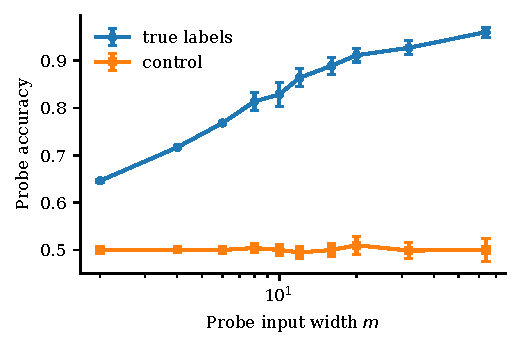
\includegraphics[width=\columnwidth]{figs/fig10_probing.pdf}
\caption{True-label and control-task probe accuracy versus probe input width (pilot, frozen random encoder).}
\label{fig:fig10_probing}
\end{figure}

\section{Discussion and Limitations}
Selectivity depends on the probe family and on the control construction, so both are fixed in advance and reported. Synthetic grammars are narrower than natural language, which limits the claims about natural text.

\section{Conclusion}
We propose a probing protocol for JEPA latents with simulated ground truth, linguistic control tasks, and selectivity reported with confidence intervals.

\section*{Acknowledgments}
The author thanks the Brazilian artificial intelligence community.

\nocite{ctl_full_names}
\bibliographystyle{IEEEtran}
\bibliography{refs}

\end{document}
